El filtro Recortar únicamente requiere copiar una cantidad $tam$ de píxeles de las esquinas de la imagen fuente para generar la imagen destino con las esquinas invertidas.

\subsubsection{Implementación en C}

Con dos ciclos anidados se recorre el área de $tam$ x $tam$ en cada esquina de la imagen fuente y se escribe en la esquina opuesta de la imagen destino.

\subsubsection{Implementación en Assembler}

También se realiza con dos ciclos anidados, pero trayendo de a 16 píxeles por vez.
En cada iteración se traen 16 píxeles de la parte A a xmm0 con la operación movups y luego se copian a la parte D, lo mismo con 16 píxeles de B en C, de C en B y de D en A. Esto puede verse en el siguiente gráfico.

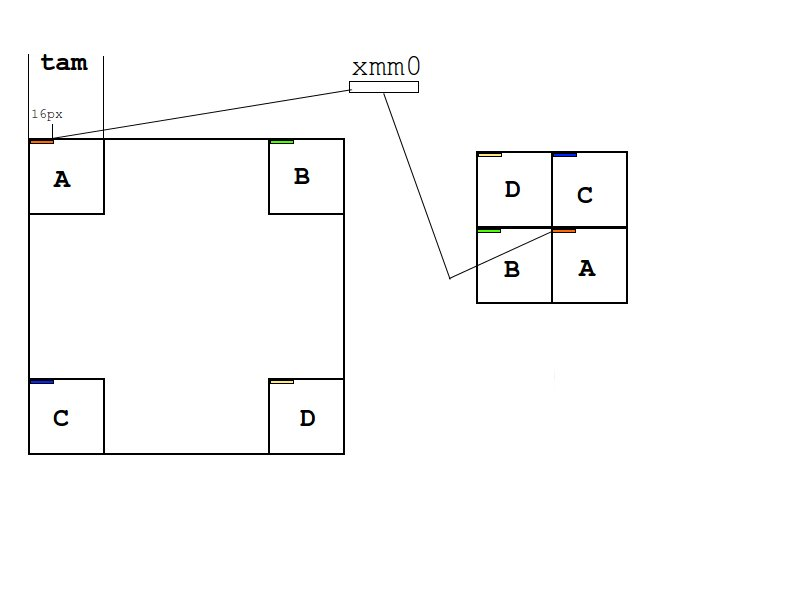
\includegraphics[width=\textwidth]{recortar.jpg} 

En el caso que $tam$ no sea múltiplo de 16, antes de entrar al ciclo se calcula el resto ($tam$ \% 16) y en la primera iteración de cada fila se suma este resto en lugar de los 16 que se suman normalmente. 

\subsubsection{Resultados}

Dado que en este filtro no se modifican los píxeles, la única diferencia debería ser en los accesos a memoria. Los ciclos en ambas implementaciones hacen 8 accesos a memoria, 4 lecturas y 4 escrituras, pero la implementación en ASM accede de a 16 bytes vs 1 de la implementación en C. 
Por lo tanto la ímplementación en C debería ser aproximadamente 16 veces más rápida.

Ejecutamos ambos filtros 1000 veces cada uno y estos son los resultados obtenidos:

\begin{center}
    \begin{tabular}{|l|l|l|}
        \hline
         & Implementación C & Implementación en asm  \\
        \hline
        Duración promedio (en ciclos de clock) & 422 596        & 24 781                 \\
        \hline
    \end{tabular}
\end{center}

Como se puede observar, la implentación en asm es $\sim$17 veces más rápida, lo que corrobora nuestra hipótesis.